\documentclass[xcolor=table,dvipsnames,svgnames,aspectratio=169]{beamer}
% Author: alick<alick9188@gmail.com>
% Author: justin <justin.w.xd@gmail.com>

% This file is modified from a solution template for:

% - Giving a talk on some subject.
% - The talk is between 15min and 45min long.
% - Style is ornate.

% Copyright 2004 by Till Tantau <tantau@users.sourceforge.net>.
%
% In principle, this file can be redistributed and/or modified under
% the terms of the GNU Public License, version 2.
%
% However, this file is supposed to be a template to be modified
% for your own needs. For this reason, if you use this file as a
% template and not specifically distribute it as part of a another
% package/program, I grant the extra permission to freely copy and
% modify this file as you see fit and even to delete this copyright
% notice.

\usepackage{tikz}
\graphicspath{{fig/}}
\mode<presentation>
{
  \usetheme{material}
  \renewcommand{\MaterialIcon}{shapepar.pdf}
  \usefonttheme[onlymath]{serif}
  \setbeamercovered{transparent=5}
  \setbeamercolor*{structure}{fg=primaryD}
  \setbeamertemplate{itemize item}{\raise1.25pt\hbox{\tikz\draw[fill=fg] (0,0) circle (.3ex);}}
  \setbeamertemplate{itemize subitem}{\color{fg}\tiny\raise1.25pt\hbox{\donotcoloroutermaths$\blacktriangleright$}}
  \setbeamertemplate{itemize subsubitem}{\raise2.5pt\hbox{\tikz\draw[fill=fg] (0,0) rectangle (.7ex, .2ex);}}

  \setlength\leftmargini{1.4em}
  \setlength\leftmarginii{1.4em}
  \setlength\leftmarginiii{1.4em}
  \setbeamersize{description width=0.24cm}

}

\usepackage{mflogo} % for \MF, \MP
\usepackage{graphicx}
\usepackage{listingsutf8}
\usepackage{xspace}
\usepackage{amsmath}
\usepackage{calligra}
\usepackage{cclicenses} % CC symbols
\usepackage{fontspec}
\usepackage[UTF8]{ctex}
\usepackage{hologo}
\usepackage{colortbl}
\usepackage{pstricks}
\usepackage{pst-node}
\usepackage{hyperxmp}
\usepackage{booktabs}
\usepackage[normalem]{ulem}
\usepackage{stackengine}
\hypersetup{
pdfauthor={Justin Wong, Alick Zhao},
pdfcopyright={Copyright (C) 2015 by Alick Zhao.
Licensed under CC-BY-SA 4.0. Some rights reserved.},
pdflicenseurl={http://creativecommons.org/licenses/by-sa/4.0/},
}

% From thuthesis user guide
\makeatletter
\def\psRotation#1(#2,#3)#4{%
  \rput{#1}(#2,#3){%
    \psellipticarc[linewidth=.4pt]{->}(0,-0.1)(0.6,0.15){120}{70}
    \ifdim#1pt>\z@\rput[l]{*0}(0.675,0){#4}\else\rput[l](0.675,0){#4}\fi
  }%
}
\makeatother

% For tipa to work.
\newfontfamily\useTIPAfont{Times New Roman}

% xeCJK conf setup
\punctstyle{kaiming}
\renewcommand\CJKfamilydefault{\CJKsfdefault} % for slides

\setCJKsansfont{WenQuanYi Micro Hei}
\setCJKmonofont{WenQuanYi Micro Hei}

\renewcommand{\TeX}{\hologo{TeX}}
\renewcommand{\LaTeX}{\hologo{LaTeX}}
\newcommand{\BibTeX}{\hologo{BibTeX}}
\newcommand{\XeTeX}{\hologo{XeTeX}}
\newcommand{\pdfTeX}{\hologo{pdfTeX}}
\renewcommand{\CTeX}{C\TeX}
\newcommand{\MiKTeX}{\hologo{MiKTeX}}
\newcommand{\MacTeX}{Mac\hologo{TeX}}
\newcommand{\beamer}{\textsc{beamer}}
\def\TeXLive{\TeX{} Live\xspace}
\let\TL=\TeXLive
\newcommand{\ThuThesis}{\textsc{ThuThesis}\xspace}

% From thuthesis user guide.
\def\cmd#1{\texttt{\color{DarkBlue}\footnotesize $\backslash$#1}}
\def\env#1{\texttt{\color{DarkBlue}\footnotesize #1}}
\def\cmdxmp#1#2#3{\small{\texttt{\color{DarkBlue}$\backslash$#1}\{#2\}\hspace{1em}\\ $\Rightarrow$\hspace{1em} {#3}\par\vskip1em}}

% For debugging.
% \includeonlyframes{current}
% \includeonly{introduction}


\lstset{
  language=[LaTeX]TeX,
	basicstyle=\ttfamily\footnotesize,
	tabsize=2,
  keywordstyle=\bfseries\ttfamily\color{primaryD},
	commentstyle=\sl\ttfamily\color[RGB]{100,100,100},
	stringstyle=\ttfamily\color[RGB]{50,50,50},
	extendedchars=true,
	breaklines=true,
}


\title
{An Introduction to \LaTeX{}}
\author[Lynn] % (optional, use only with lots of authors)
{刘思林\\ \texttt{liusilinlynn@hotmail.com}}

\institute{Chongqing University of Posts and Telecommunications}
% - Use the \inst command only if there are several affiliations.
% - Keep it simple, no one is interested in your street address.

\date[小组内部培训] % (optional)
{2017 年 6 月 4 日}

\subject{LaTeX, paper, ThuThesis}

% Delete this, if you do not want the table of contents to pop up at
% the beginning of each subsection:
\AtBeginSubsection[]
{
  \begin{frame}<beamer>{目录}
    \tableofcontents[currentsection,currentsubsection]
  \end{frame}
}


% If you wish to uncover everything in a step-wise fashion, uncomment
% the following command:

%\beamerdefaultoverlayspecification{<+->}

\hypersetup{
%pdfpagemode=FullScreen,
}

\logo{
\includegraphics[height=.15\textheight]{cqupt.jpg}}

\begin{document}

\begin{frame}
  \titlepage
\end{frame}

\begin{frame}{目录}
  \tableofcontents
  % You might wish to add the option [pausesections]
\end{frame}


% Since this a solution template for a generic talk, very little can
% be said about how it should be structured. However, the talk length
% of between 15min and 45min and the theme suggest that you stick to
% the following rules:

% - Exactly two or three sections (other than the summary).
% - At *most* three subsections per section.
% - Talk about 30s to 2min per frame. So there should be between about
%   15 and 30 frames, all told.

\section{简介}
\subsection{\TeX 与 \LaTeX}

\begin{frame}[fragile]{\TeX 与 \LaTeX}
  % TODO: photo of Knuth & Lamport
  \begin{columns}[T]
    \column{.8\textwidth}
    \begin{itemize}
      \item \TeX: $\tau\varepsilon\chi$ (\textipa{/'tEx/},
        \textipa{/'tEk/})
        \begin{itemize}
          \item 生成精美图书的排版系统,由高德纳 (Donald E.~Knuth) 于开发
          \item 发音接近``泰赫'',''泰克'',而非``泰克斯''
          \item 最新版本为 \TeX\ 3.14159265,漂亮、美观、稳定、通用,尤其擅长数学公式排版
        \end{itemize}
      \item \LaTeX\ (\textipa{/'la:tEx/}, \textipa{/'leItEk/})
        \begin{itemize}
          \item 后人在 \TeX 的基础上的宏包
          \item 降低使用门槛极其丰富的宏包、模板 
          \item 提供扩展功能广泛用于学术界,期刊会议论文模板、大学学位论文模板
        \end{itemize}
    \end{itemize}
    \column{.2\textwidth}
    \vspace*{10mm}
    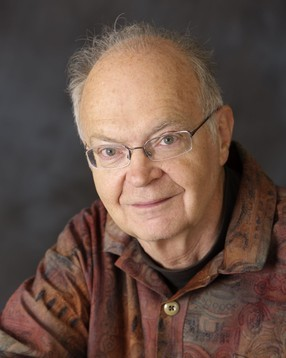
\includegraphics[width=\textwidth]{Knuth.jpg}

    %\vspace*{5mm}
    %\includegraphics[width=\textwidth]{Lamport.jpg}
      
  \end{columns}
\end{frame}

\begin{frame}{和 Word 对比}
  \begin{table}[h]
    \centering
    \rowcolors[]{1}{primaryL}{primaryL!40}
    \begin{tabular}{r|l}
      Microsoft\textsuperscript{\textregistered}  Word & \LaTeX \\
      \hline
      文字处理工具 & 专业排版软件 \\
      容易上手,简单直观 & 需要一定的门槛 \\
      所见即所得 & 所见即所想,所想即所得 \\
      高级功能不易掌握 & 进阶难,但一般用不到 \\
      处理长文档需要丰富经验 & 和短文档处理基本无异 \\
      花费大量时间调格式 & 无需担心格式,专心作者内容 \\
      公式排版差强人意 & 尤其擅长公式排版 \\
      二进制格式,兼容性差 & 文本文件,易读、稳定 \\
      付费商业许可 & 自由免费使用 \\
    \end{tabular}
  \end{table}
\end{frame}

\begin{frame}{\TeX{}排版举例:公式}
  \begin{exampleblock}{无编号公式}
    \begin{equation*}
      \mathcal{F}(\xi)=\int_{-\infty}^{\infty}\!\!
      f(x)\mathrm{e}^{-\mathrm{j}2\pi \xi x}\,\mathrm{d}x
    \end{equation*}
  \end{exampleblock}
  \begin{exampleblock}{多行多列公式}
    % Taken from Mathmode.tex
    \begin{align}
      y & =d & z & =1\\
      y & =cx+d & z & =x+1\\
      y_{12} & =bx^{2}+cx+d & z & =x^{2}+x+1\nonumber \\
      y(x) & =ax^{3}+bx^{2}+cx+d & z & =x^{3}+x^{2}+x+1
    \end{align}
  \end{exampleblock}
\end{frame}

\begin{frame}{\TeX{}排版举例:公式}
  \begin{exampleblock}{编号多行公式}
    % Taken from Mathmode.tex
    \begin{multline}
    A=\lim_{n\rightarrow\infty}\Delta x\left(a^{2}+\left(a^{2}+2a\Delta x+\left(\Delta x\right)^{2}\right)\right.\label{eq:reset}\\
    +\left(a^{2}+2\cdot2a\Delta x+2^{2}\left(\Delta x\right)^{2}\right)\\
    +\left(a^{2}+2\cdot3a\Delta x+3^{2}\left(\Delta x\right)^{2}\right)\\
    +\ldots\\
    \left.+\left(a^{2}+2\cdot(n-1)a\Delta x+(n-1)^{2}\left(\Delta x\right)^{2}\right)\right)\\
    =\frac{1}{3}\left(b^{3}-a^{3}\right)
  \end{multline}
\end{exampleblock}
\end{frame}

\begin{frame}{\TeX{}排版举例:图形}
  % From thuthesis user guide.
  \begin{minipage}[c]{0.3\linewidth}
    \psset{unit=0.8cm}
    \begin{pspicture}(-1.75,-3)(3.25,4)
      \psline[linewidth=0.25pt](0,0)(0,4)
      \rput[tl]{0}(0.2,2){$\vec e_z$}
      \rput[tr]{0}(-0.9,1.4){$\vec e$}
      \rput[tl]{0}(2.8,-1.1){$\vec C_{ptm{ext}}$}
      \rput[br]{0}(-0.3,2.1){$\theta$}
      \rput{25}(0,0){%
      \psframe[fillstyle=solid,fillcolor=lightgray,linewidth=.8pt](-0.1,-3.2)(0.1,0)}
      \rput{25}(0,0){%
      \psellipse[fillstyle=solid,fillcolor=yellow,linewidth=3pt](0,0)(1.5,0.5)}
      \rput{25}(0,0){%
      \psframe[fillstyle=solid,fillcolor=lightgray,linewidth=.8pt](-0.1,0)(0.1,3.2)}
      \rput{25}(0,0){\psline[linecolor=red,linewidth=1.5pt]{->}(0,0)(0.,2)}
      \psRotation{0}(0,3.5){$\dot\phi$}
      \psRotation{25}(-1.2,2.6){$\dot\psi$}
      \psline[linecolor=red,linewidth=1.25pt]{->}(0,0)(0,2)
      \psline[linecolor=red,linewidth=1.25pt]{->}(0,0)(3,-1)
      \psline[linecolor=red,linewidth=1.25pt]{->}(0,0)(2.85,-0.95)
      \psarc{->}{2.1}{90}{112.5}
      \rput[bl](.1,.01){C}
    \end{pspicture}
  \end{minipage}\hspace{1cm}
  \begin{minipage}[t]{0.5\linewidth}
    \psset{unit=0.3cm}
    \begin{pspicture}(1,2)(18,14)
      %\psgrid[gridcolor=lightgray,subgriddiv=0,subgridcolor=lightgray]
      %
      \psline[linewidth=1pt,linecolor=black](6,0.5)(6,14)
      \psline[linewidth=1pt,linecolor=black](1,8.5)(6,7)
      \psline[linewidth=1pt,linecolor=black](1.5,5.5)(11,8.5)
      %
      \rput(17,3){$x$}
      \rput(5.5,13){$y$}
      \rput(10.5,8.75){$z$}
      \rput(11,7.1){$\vec{r}$}
      %
      \psline[linewidth=1.5pt,linecolor=black]{<->}(6,7)(6,11.25)
      \rput(5.35,9.4){$R$}
      \psline[linewidth=1.5pt,linecolor=Green]{->}(6.5,12)(4.75,12)
      \rput(7.5,12.8){ $I d\vec{l}$}
      %
      \psellipse[doubleline=true,doublecolor=yellow,doublesep=3pt,linecolor=blue](6,7)(3,4.5)
      \psline[linewidth=1pt,linecolor=black](6,7)(17.5,3.5)
      \psline[linewidth=1.5pt,linecolor=black]{->}(6,11.38)(11.95,5.225)
      %
      \psarc[linewidth=1.5pt,linecolor=gray](6,8){3.4}{85}{95}
      %
      \psline[linewidth=1.5pt,linecolor=gray]{->}(12,5.15)(12,8.15)
      \psline[linewidth=1.5pt,linecolor=black]{->}(12,5.15)(15,7.25)
      \psline[linewidth=1.5pt,linecolor=gray]{->}(12,5.15)(15,4.25)
      %
      \psline[linewidth=1pt,linecolor=black](12,8.15)(15,7.25)(15,4.25)
      %
      \Cnode*[linecolor=black,radius=0.1cm](12,5.15){a}
      \rput(11.5,4.5){ $P$}
      %
      \rput(12.5,8.9){$dB_y$}
      \rput(14.5,3.4){$dB_x$}
      \rput(15.5,8){ $d \boldmath{\vec{B}}$}
      %
      \psarc[linewidth=1pt]{<->}(12,5){5.5}{133}{161}
      \rput(7.2,8.5){ $\theta$}
    \end{pspicture}
    \medskip

    %\hspace{2cm}
    \begin{figure}[h]
      \centering
      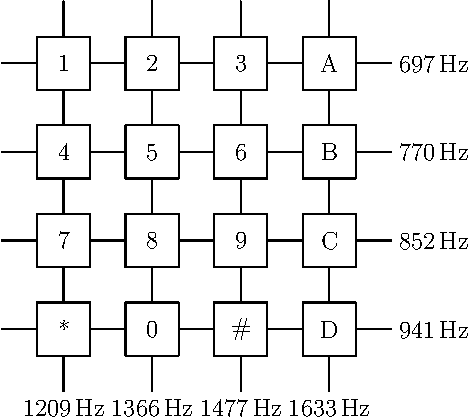
\includegraphics[height=.33\textheight]{dtmf.pdf}
    \end{figure}
  \end{minipage}
\end{frame}

\begin{frame}{\TeX{}排版举例:文档}
  \begin{columns}
    \begin{column}{.45\textwidth}
      \begin{figure}[h]
        \centering
        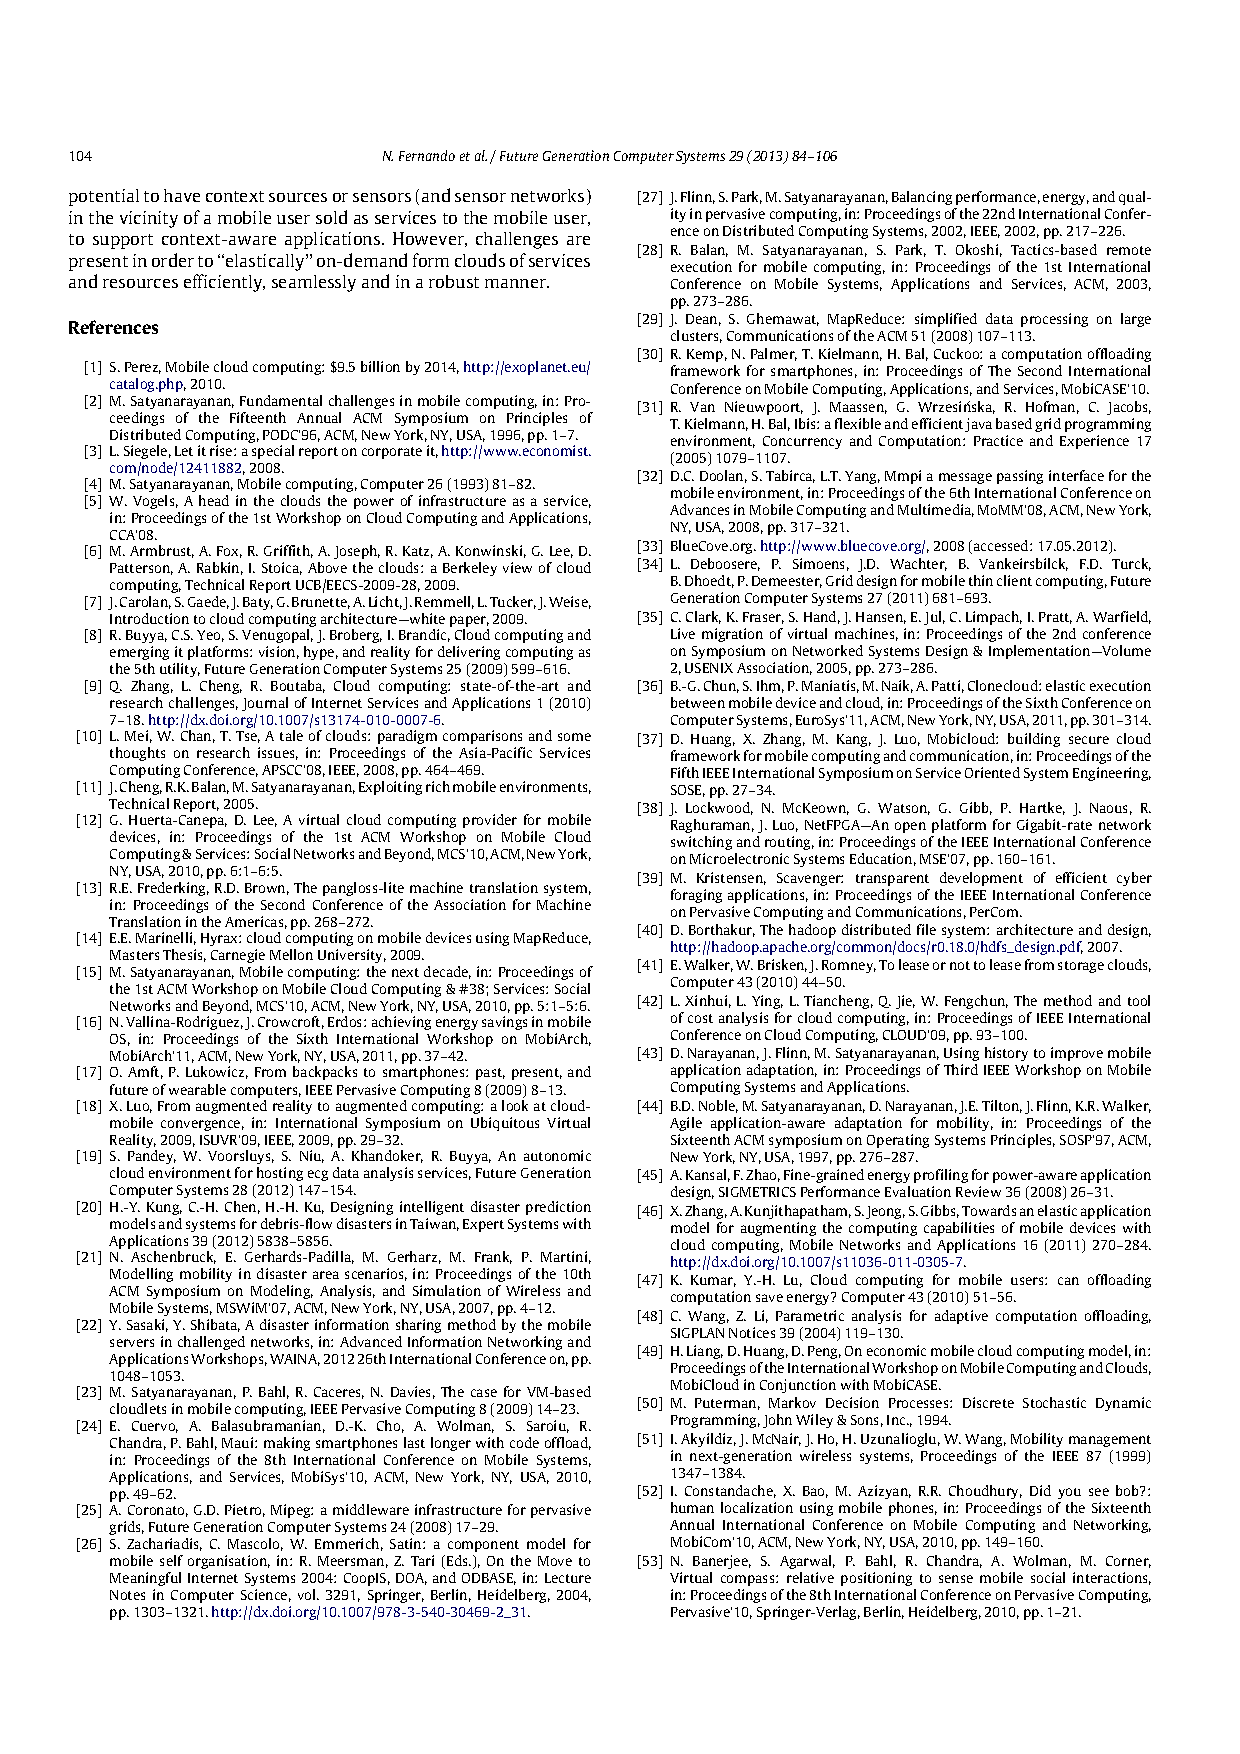
\includegraphics[width=.8\textwidth]{references.pdf}
      \end{figure}
    \end{column}
    \begin{column}{.45\textwidth}
      \begin{figure}[h]
        \centering
        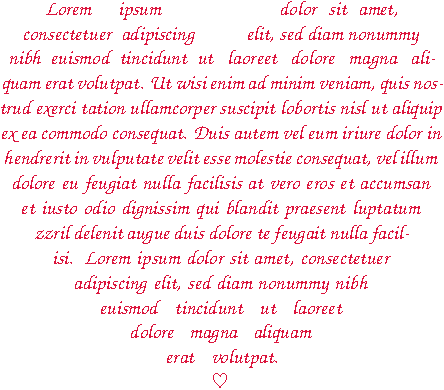
\includegraphics[width=.8\textwidth]{shapepar.pdf}
      \end{figure}
    \end{column}
  \end{columns}
\end{frame}

\begin{frame}{\TeX{}排版举例:幻灯片}
  \begin{columns}
    \begin{column}{.45\textwidth}
      \begin{figure}[h]
        \centering
        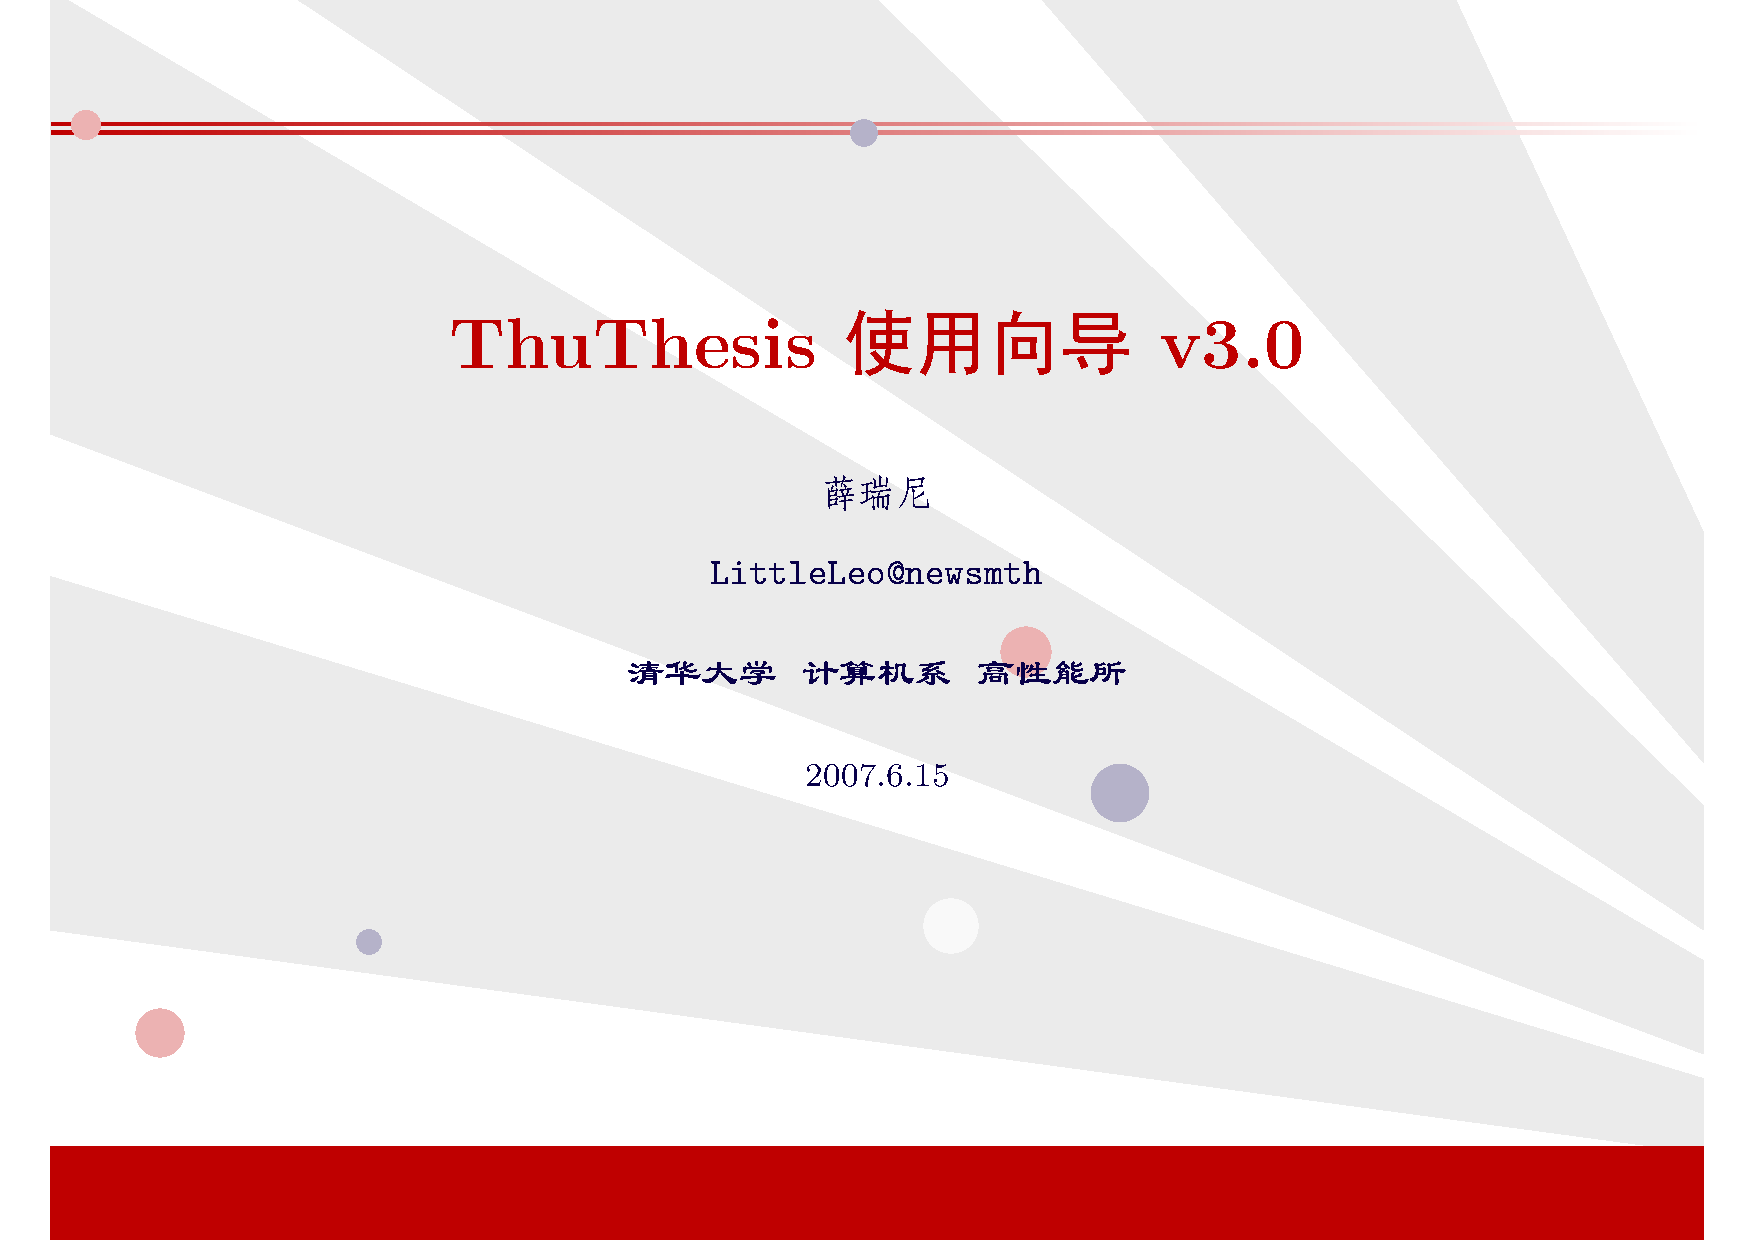
\includegraphics[width=\textwidth]{slides-powerdot.pdf}
      \end{figure}
    \end{column}
    \begin{column}{.45\textwidth}
      \begin{figure}[h]
        \centering
        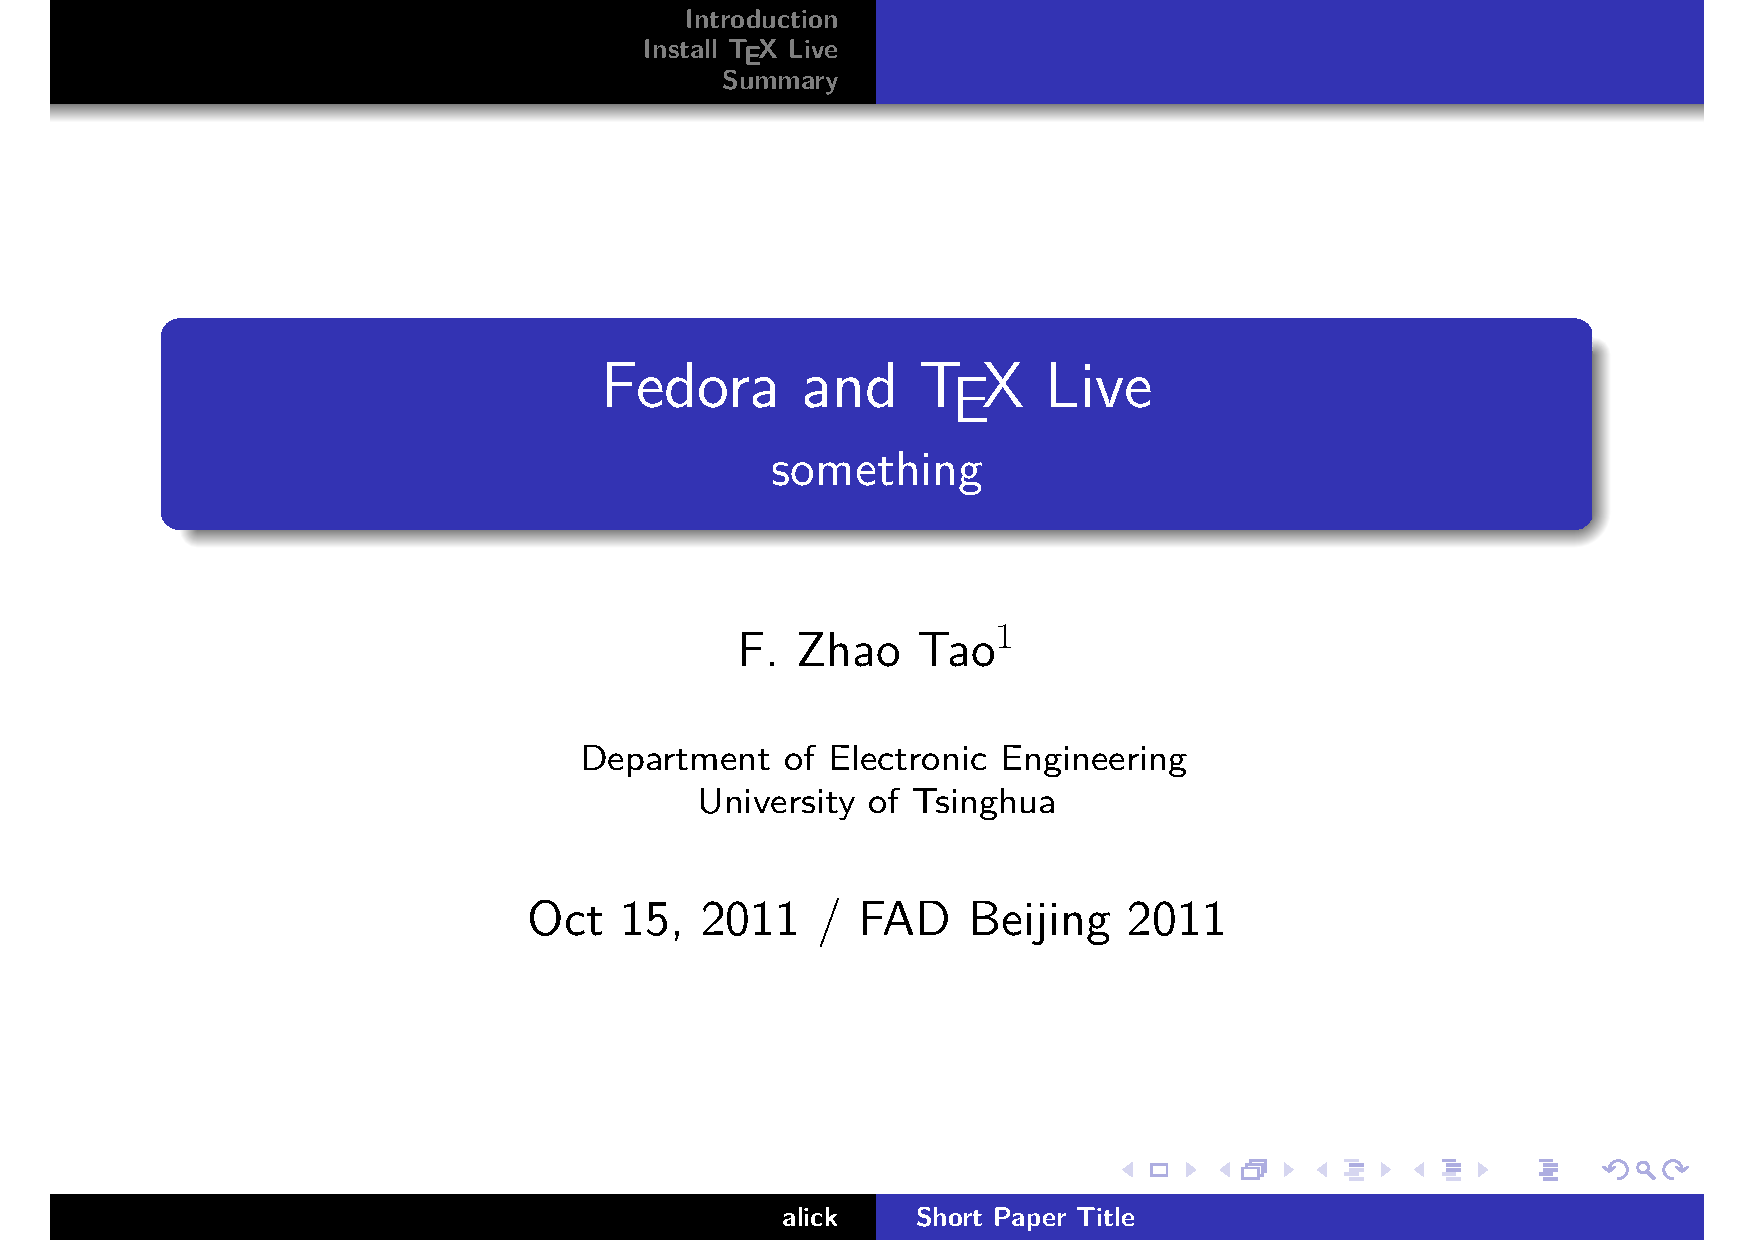
\includegraphics[width=\textwidth]{slides-beamer.pdf}
      \end{figure}
    \end{column}
  \end{columns}
\end{frame}

\subsection{\LaTeX{} 的获取安装}

%\begin{frame}{如何安装 \hologo{(La)TeX}?}
  
%\end{frame}

\begin{frame}[fragile]
  \frametitle{安装镜像下载}
  \LaTeX{}的发行版包括很多版本,这里我们选择的发行版本是 \TL 
  \begin{itemize}
    \item 为什么选择 \TL 发行版?
      \begin{itemize}
        \item 跨平台:Windows,Linux,Mac OS
        \item 即时更新,稳定的开源社区,工具集完整
      \end{itemize}
    \item 离线安装镜像 (约3GB大小)
      \begin{itemize}
        \item {\footnotesize
          \url{https://mirrors.tuna.tsinghua.edu.cn/CTAN/systems/texlive/Images/texlive.iso}}
        \item {\footnotesize
          \url{https://mirrors.aliyun.com/CTAN/systems/texlive/Images/texlive.iso}}
      \end{itemize}
    \item 注意!!! 
      \begin{itemize}
         \item 镜像文件的安装使用虚拟光驱,尽量不要解压缩
         \item 截图……
      \end{itemize}
  \end{itemize}   
\end{frame}


\begin{frame}[fragile]
\frametitle{镜像的安装}
  \begin{figure}[h]
    \centering
    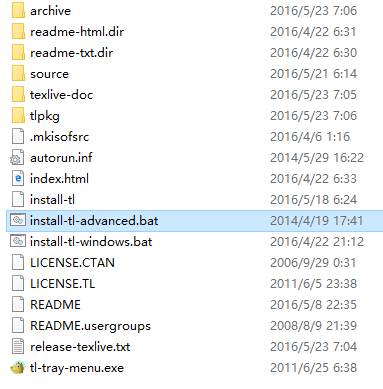
\includegraphics[scale=0.7]{install0.png}
  \end{figure}
\end{frame}

\begin{frame}[fragile]
  \begin{figure}[h]
    \centering
    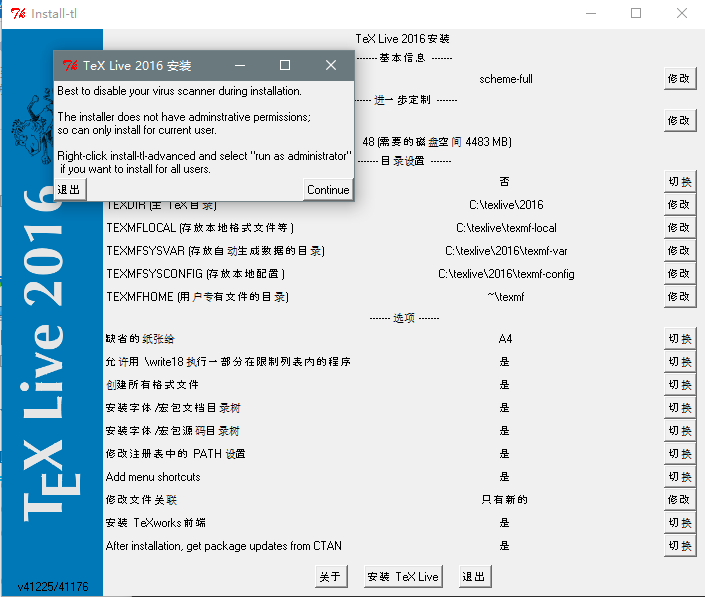
\includegraphics[scale=0.45]{install.png}
  \end{figure}
   \centering Windows 上安装过程比较慢,尤其是最后的生成索引阶段,请耐心等待
\end{frame}


\begin{frame}[fragile]
  \frametitle{安装后测试}

  \begin{itemize}
    \item 编辑 \texttt{hello.tex} (Windows 下不要用中文文件名;注意
      \LaTeX{} 文档对大小写敏感。)
      \lstset{language=[LaTeX]TeX}
      \begin{card} \begin{lstlisting}[basicstyle=\ttfamily]
\documentclass{article}
\usepackage{ctex}  % 加入中文支持
\begin{document}
\TeX{}你好!
\end{document}
        \end{lstlisting}\end{card}
      \begin{itemize}
        \item Windows 下缺省使用中易字体
        \item Linux、Mac OS X 下需要注意字体(参见 ctex 文档)
      \end{itemize}
    \item 使用 XeLaTeX 引擎编译,得到 PDF 文档
      \begin{center}
        \fbox{\textrm \TeX{}\songti 你好!}
      \end{center}
  \end{itemize}
\end{frame}

%%% vim: set ts=2 sts=2 sw=2 isk+=\: et tw=80 cc=+1 formatoptions+=mM:

\include{basis}
%\include{thuthesis}
\section{总结}

\subsection{常见问题}

\begin{frame}{常见问题}
  \begin{itemize}
    \item \alert{编译不通过} 缺少必要宏包,命令拼写错误,括号未配对等
    \item \alert{表格图片乱跑} \LaTeX{} 自身的浮动定位算法
    \item \alert{段落间距变大} \LaTeX{} 排版算法
    \item \alert{参考文献} 推荐使用 \BibTeX{},也可以手写 \cmd{bibitem}
  \end{itemize}
\end{frame}

\subsection{学习资源}

\begin{frame}{系统学习}
  \begin{itemize}
      \item 包太雷 《\LaTeX{} Notes(第二版)》~(3小时)
      \item Stefan Kottwitz 《LaTeX Cookbook》
      \item WikiBooks
        \begin{itemize}
          \item \url{https://en.wikibooks.org/wiki/LaTeX}
          \item \url{https://zh.wikibooks.org/wiki/LaTeX}
        \end{itemize}
      \item 经典文档
        \begin{itemize}
          \item 仔细阅读《一份不太简短的~\LaTeXe{} 介绍》(lshort-zh)~(1--2 天)
          \item 粗略阅读《\LaTeXe{} 插图指南》~(2--3 小时)
        \end{itemize}
      %\item 仔细阅读《\ThuThesis{} 用户手册》~(20 分钟)
      %\item 从~\ThuThesis{} 示例文档入手
  \end{itemize}
\end{frame}

\begin{frame}{扩展阅读}
  \begin{itemize}
    \item 一份其实很短的 \LaTeX 入门文档 (Liam Huang) \\
      \url{http://liam0205.me/2014/09/08/latex-introduction/} 
    \item 网站推荐: 
      \begin{itemize}
        \item http://www.latexstudio.net/
        \item http://www.chinatex.org/
      \end{itemize}
    \item 知乎专栏: http://zhuanlan.zhihu.com/LaTeX
    %\item \ThuThesis{}使用向导 v3.0 (薛瑞尼)
    \item \LaTeX{}杂谈(刘海洋)
    \item 《\LaTeX{}入门》(刘海洋)
    \item \LaTeX\ Tips:
      \url{https://alick.fedorapeople.org/fudcon-apac-2014/latex-tips.pdf}
    \item Linux 用户:\url{https://github.com/alick/fad-texlive-talk}
  \end{itemize}
\end{frame}


\begin{frame}{利用文档}
  \begin{itemize}
    \item 常用文档
      \begin{itemize}
        \item symbols: 符号大全
        \item Mathmode: 数学参考
        \item ctex, xeCJK: 中文支持
        \item texlive-zh: \TL 安装与使用
        \item 所用宏包文档
      \end{itemize}
    \item 工具
      \begin{itemize}
        \item tlmgr: \TL 管理器
        \item texdoc: \TeX{} 文档查看器\\
          例如:\texttt{texdoc lshort-zh}
        \item \url{http://texdoc.net/}
        \item TeX Studio 和 WinEdt 都支持在帮助里看文档
      \end{itemize}
  \end{itemize}
\end{frame}

\begin{frame}{一点人生的经验}
  \begin{itemize}
    \item 不要过于相信网上的中文文档
      \begin{itemize}
        \item 简单鉴别方法: 排版的好看程度
      \end{itemize}
    %\item 湿兄用U盘拷给你的的ctex套装一定是过时的,ThuThesis 八成是老版本的
    \item 如果你要处理中文
      \begin{itemize}
        \item 使用 XeLaTeX, 使用 XeLaTeX, 使用 XeLaTeX
        \item 忘记 CJK, 忘记 CJK, 忘记 CJK
        \item 使用 xeCJK
        \item 使用 ctex 宏包(2.0以上版本) (跟 C\TeX 套装仅仅是名字像)
      \end{itemize}
    \item 写一点,编译一次,减小排错搜索空间
  \end{itemize} 
\end{frame}

% 寻求帮助
\begin{frame}{求助}
  \begin{columns}[c]
    \begin{column}{.45\textwidth}
      \begin{itemize}
        \item BBS
          \begin{itemize}
            %\item \href{http://www.newsmth.net/nForum/board/TeX}{水木
             % 社区 TeX 版}
            \item \href{http://bbs.ctex.org/}{bbs.ctex.org}
          \end{itemize}
        \item \href{http://www.tex.ac.uk/cgi-bin/texfaq2html}{UK FAQ}
        \item TeX StackExchange
        \item \href{http://justfuckinggoogleit.com/}{Google}
          \begin{itemize}
            \item 使用英语搜索
          \end{itemize}
      \end{itemize}
    \end{column}
    \begin{column}{.45\textwidth}
      
\includegraphics[width=\textwidth]{TFZsuperellipse-crop.pdf}
    \end{column}
  \end{columns}
\end{frame}

\begin{frame}{你也可以帮助}
  \begin{itemize}
    \item 错误反馈:GitHub Issues
    \item 改进建议:GitHub Issues
    \item 出力维护:LaTeX 宏包编写、Git
    \item 科普、答疑%\pause \hspace{2em}\alert{图书馆讲座征主讲人!}
  \end{itemize}
\end{frame}

%%% vim: set ts=2 sts=2 sw=2 isk+=\: et tw=80 cc=+1 formatoptions+=mM:


\section*{附录}


\begin{frame}
  \begin{itemize}
    \item 本幻灯片
      \begin{itemize}
        %\item \url{https://github.com/tuna/thulib-latex-talk}
        \item \url{https://www.overleaf.com/read/bdynvrzpqmwq}
        % \item Overleaf 版本有只包含第一章、
        \item 表示感谢
      \end{itemize}
    \item 本幻灯片基于:
      \begin{itemize}
        \item \url{http://github.com/alick/fad-texlive-talk}
        \item \ThuThesis{}使用向导 v3.0
      \end{itemize}
    \item 许可证:CC BY-SA 4.0 Unported \cc\ccby\ccsa
  \end{itemize}
\end{frame}

\begin{frame}
  \begin{center}
    {\Huge\calligra Thank you!}
  \end{center}
\end{frame}

\end{document}

%%% vim: set ts=2 sts=2 sw=2 isk+=\: et tw=80 cc=+1 formatoptions+=mM:
